% !TeX root=../main.tex
\section{Покращення асимптотичної оцінки}

Нескладно помітити, що $\mu_{p}(x) = C x - \frac{1-C}{1 - p}$ є розв'язком рівняння \eqref{eq:model_equation} $\forall C \in \RR$:
\begin{align*}
&1 + \frac{2 (1-p)}{x} \int_{0}^{x} \mu_{p}(t) dt + p\mu_{p}(x) = \\
&=1 + \frac{2 (1-p)}{x} \int_{0}^{x} \left\{C t - \frac{1 - C}{1 - p} \right\} dt + p \left( C x - \frac{1 - C}{1 - p}\right) = \\
&=1 + (1 - p) C x - 2(1 - C) + p C x - (\frac{1}{1 - p} - 1)(1 - C) = \\
&= C(x + 1) - \frac{1 - C}{1 - p} = \mu_{p}(x+1).
\end{align*}

Тому резонно апроксимувати досліджувану функцію $m_{p}(x)$ використовуючи функцію $\mu_{p}$. Далі буде доведено наступне твердження:
\begin{equation}
\label{eq:fine_asymptotics_1}
\lim\limits_{x \rightarrow \infty} \left( m(x) - C_{p} x + \frac{1 - C_{p}}{1 - p} \right) = 0.
\end{equation}

\subsection{Застосування тауберівської теореми для покращення оцінки}

Нескладно помітити, що

\begin{equation}
\label{eq:q_p_transform}
\begin{split}
Q_{p}(s) = \int\limits_{1}^{s} \frac{1-p}{u(e^u - p)} du =& \int\limits_{1}^{s} \frac{1}{u} du - \int\limits_{1}^{s} \frac{e^u -1}{u(e^u - p)} du = \\
=& \ln(s) - \int\limits_{1}^{s} \frac{e^u -1}{u(e^u - p)} du.
\end{split}
\end{equation}

Тоді з \eqref{eq:q_p_transform} та \eqref{eq:model_laplace_sol} маємо

\begin{gather*}
M_{p}(s) =\frac{e^{-2Q_p(s)}}{(e^s - p)} \int\limits_s^\infty \frac{e^{2Q_p(u)}}{u^2} du = \\
\frac{s^{-2}}{e^s-p} \exp \left(2 \int\limits_{1}^{s} \frac{e^u -1}{u(e^u - p)} du\right) \int\limits_s^\infty \exp\left(-2 \int\limits_{1}^{u} \frac{e^\tau -1}{\tau(e^\tau - p)} d\tau\right) du.
\end{gather*}

Оскільки $e^u - 1 \sim u,~u \rightarrow 0$, то інтеграл $\int\limits_{0}^{1} \frac{e^u -1}{u(e^u - p)} du$ існує для $\forall p < 1$. Отже, можна винести з-під інтегралу константу $\exp\left(\int\limits_{0}^{1} \frac{e^u -1}{u(e^u - p)} du\right)$.

\begin{gather*}
M_{p}(s) = \frac{s^{-2}}{e^s-p} \exp \left(2 \int\limits_{0}^{s} \frac{e^u -1}{u(e^u - p)} du\right) \int\limits_s^\infty \exp\left(-2 \int\limits_{0}^{u} \frac{e^\tau -1}{\tau(e^\tau - p)} d\tau\right) du = \\
\begin{align*}
=\frac{s^{-2}}{e^s-p} \exp \left(2 \int\limits_{0}^{s} \frac{e^u -1}{u(e^u - p)} du\right) & \left[\rule{0cm}{1.05cm} (1-p) C_{p} - \right. \\
& \left.- \int\limits_0^s \exp\left(-2 \int\limits_{0}^{u} \frac{e^\tau -1}{\tau(e^\tau - p)} d\tau\right) du \right]
\end{align*}
\end{gather*}

Оскільки $s^2 M_{p}(s)$ --- аналітична функція на $\operatorname{\mathfrak{Re}} s > \sigma$, де $\sigma < 0$ при $p < 1$, то з розкладу в ряд Тейлора випливає
\begin{equation}
M_{p}(s) = \frac{C_{p}}{s^2} + \frac{\frac{\partial}{\partial s}(s^2 M_{p}(s))}{s} + \psi_{p}(s),
\end{equation}
де $\psi_{p}(s)$ --- аналітична на $\operatorname{\mathfrak{Re}} s > \sigma$. Позначимо через $R_{p}(s)=\int\limits_{0}^{s} \frac{e^u -1}{u(e^u - p)} du$, тоді
\begin{gather*}
\frac{\partial}{\partial s}(s^2 M_{p}(s)) = -\frac{e^s}{(e^s - p)^2} \left[(1-p) C_{p} e^{2 R_{p}(s)} - \int\limits_{0}^{s} e^{2(R_{p}(s) - R_{p}(u))} du\right] + \\
+ \frac{1}{e^s - p} \left[ \left((1 - p) C_{p} - \int\limits_{0}^{s} e^{- R_{p}(u))} du\right) e^{2R_{p}(s)} \frac{2(e^s - 1)}{s(e^s - p)} - e^{2(R_{p}(s) - R_{p}(s))} \right] 
\end{gather*}
Підставивши $s = 0$, отримаємо
\begin{equation*}
\frac{\partial (s^2 M_{p})}{\partial s}(0) = -\frac{1}{(1-p)^2} (1-p) C_{p} + \frac{1}{1-p} \left[ 2 C_{p} - 0 - 1 \right] = \frac{C_{p} - 1}{1 - p}.
\end{equation*}
Таким чином,
\begin{equation}
\label{eq:model_laplace_taylor}
M_{p}(s) = C_{p} s^{-2} - \frac{1 - C_{p}}{1 - p} s^{-1} + \psi_{p}(s).
\end{equation}
Розглянемо перетворення Лапласа від $m_{p}(x) - C_{p} x$:
\begin{gather*}
\Lapl{m_{p}(x) - C_{p} x}  = M_{p}(s) - C_{p} s^{-2} =  \frac{C_{p} - 1}{1 - p} s^{-1} + \psi_{p}(s), \\
\lim\limits_{s \rightarrow 0} \frac{\Lapl{m_{p}(x) - C_{p} x}}{s^{-1}} = \frac{C_{p} - 1}{1 - p}.
\end{gather*}
Тоді за тауберівською теоремою \eqref{eq:tauber_thm} можна зробити висновок
\begin{equation}
\lim\limits_{x \rightarrow \infty} m_{p}(x) - C_{p} x = \frac{C_{p} - 1}{1 - p},
\end{equation}
тобто \eqref{eq:fine_asymptotics_1} доведено.

\subsection{Застосування зворотної формули Фур'є-Мелліна}

У цьому параграфі буде виконано уточнення оцінки \eqref{eq:fine_asymptotics_1} за допомогою зворотної формули Фур'є-Мелліна. У роботі \cite{schiff1999laplace} цей результат сформульовано наступним чином.
\begin{thm}[Формула Фур'є-Мелліна]
\label{eq:mellin_thm}
Нехай $f(t) = 0, t < 0$,  $f(t) < Ce^{\alpha t}$, $\Lapl{f(t)} = F(s)$. Тоді $\forall \sigma > \alpha$
\begin{equation}
f(t) = \frac{1}{2\pi i}\int\limits_{\sigma - i\infty}^{\sigma + i\infty} e^{st} F(s) ds.
\end{equation}
\end{thm}
\begin{corollary}
\label{eq:mellin_analytic}
Нехай $0 < f(t) < Ce^{\alpha t}, ~ \forall \alpha > 0$ і $F(s)$ --- аналітична в півплощині $s > \sigma, ~\sigma < 0$. Тоді
\begin{equation}
f(t) = \frac{1}{2\pi i}\int\limits_{- i\infty}^{+ i\infty} e^{st} F(s) ds.
\end{equation}
\begin{proof}
Спочатку покажемо, що $|F(s)| < F(\operatorname{\mathfrak{Re}} s)$.
\begin{equation*}
|F(s)| = \left| \int\limits_{0}^{\infty}  f(t) e^{-st} dt \right| \leq \int\limits_{0}^{\infty} \left|f(t) e^{-st} \right| dt = \int\limits_{0}^{\infty} f(t)  e^{-t\operatorname{\mathfrak{Re}} s}  dt = F(\operatorname{\mathfrak{Re}} s).
\end{equation*}
Тепер, оскільки $F$ --- аналітична в правій півплощині відносно $\sigma$, то за теоремою Коші \cite{lavrentiev1965}
\begin{figure}[h]
	\centering
	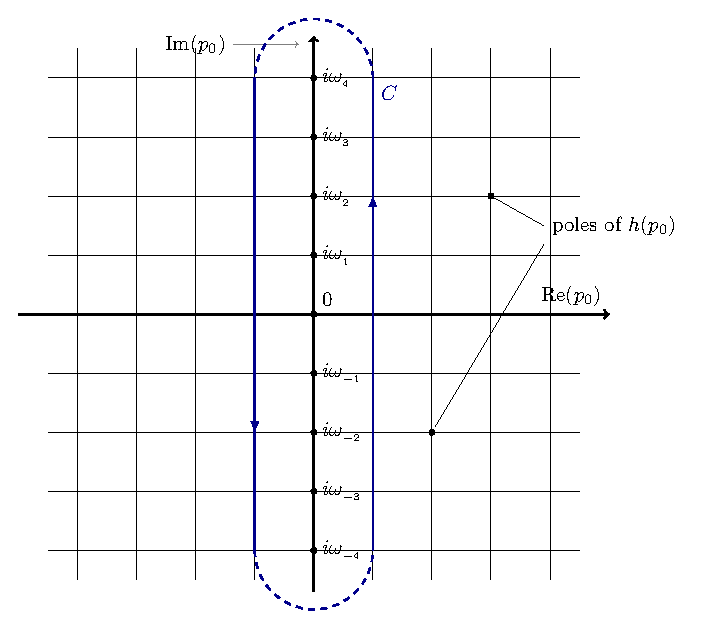
\includegraphics{chapter_Asymptotics/img/contour_bar}
	\caption{Шлях інтегрування аналітичної функції $F(s)$}
\end{figure}
\begin{equation*}
\int\limits_{-i\infty}^{i\infty} F(s) e^{st} ds + \int\limits_{iR}^{iR + \delta} F(s) e^{st} ds + \int\limits_{iR + \delta}^{-iR + \delta} F(s) e^{st} ds + \int\limits_{-iR + \delta}^{-iR} F(s) e^{st} ds = 0.
\end{equation*}
Позначимо $V(R)=\int\limits_{-iR + \delta}^{iR + \delta} F(s) e^{st} ds, ~\forall 0 < \delta < 1$. Нескладно переконатися, що 
$|\int\limits_{iR}^{iR + \delta} F(s) e^{st} ds| \leq \delta e^{\delta t} \max\limits_{[0,1]} |F(\operatorname{\mathfrak{Re}} s)| \leq \delta \cdot const$. Тоді $\forall \delta > 0, ~\forall R > 0$
\begin{equation*}
\left|~\int\limits_{-iR}^{iR} F(s) e^{st} ds - V(R)\right| \leq \delta \cdot const.
\end{equation*}
Зробимо граничний перехід $\delta \rightarrow 0$: оскільки через аналітичність $F(s)$ інтеграл $\int\limits_{-iR}^{iR} F(s) e^{st} ds$ існує, то
\begin{equation*}
\int\limits_{-iR}^{iR} F(s) e^{st} ds = V(R).
\end{equation*}
Завершується доведення граничним переходом $R \rightarrow \infty$:
\begin{equation*}
\lim\limits_{R \rightarrow \infty} \frac{1}{2\pi i} \int\limits_{-iR}^{iR} F(s) e^{st} ds =\lim\limits_{R \rightarrow \infty}\frac{1}{2\pi i} V(R) = f(t).
\end{equation*}
\end{proof}
\end{corollary}

Виходячи з рівняння \eqref{eq:model_laplace_taylor}, аналітичності $\psi_{p} (s)$ та наслідку \eqref{eq:mellin_analytic}, маємо наступне тверждення:
\begin{equation}
m_{p}(x) = \frac{1}{2\pi i} \int\limits_{\delta - i\infty}^{\delta + i\infty} M_{p}(s) e^{sx} ds = C_{p} x - \frac{1 - C_p}{1-p} + \frac{1}{2\pi} \int\limits_{-R}^{R} \psi_{p}(it) e^{itx} dt.
\end{equation}

\begin{lem}
Для $\forall p \in [0; 1)$
\begin{equation}
\psi_{p}(it) \sim O\left(\frac{1}{|t|}\right)
\end{equation}
\begin{proof}
Якщо показати, що $M_{p}(it) = O\left(\frac{1}{|t|}\right)$, то твердження леми випливає автоматично:
\begin{equation*}
\psi_{p}(it)=M_{p}(it) + C_{p} t^{-2} - i \frac{1-C_{p}}{1 - p} t^{-1} = O\left(\frac{1}{|t|}\right)
\end{equation*}
Залишається показати, що для
\begin{equation*}
M_{p}(s) = \frac{s^{-2}}{e^s-p} \exp \left(2 \int\limits_{0}^{s} \frac{e^u -1}{u(e^u - p)} du\right) \int\limits_s^\infty \exp\left(-2 \int\limits_{0}^{u} \frac{e^\tau -1}{\tau(e^\tau - p)} d\tau\right) du 
\end{equation*}
твердження правдиве. Щоб при підрахунку $M_{p}(it)$ інтегрувати за уявною віссю, необхідно показати, що інтеграл
\begin{equation*}
\int\limits_{it}^{i\infty} \exp\left(-2 \int\limits_{0}^{u} \frac{e^\tau -1}{\tau(e^\tau - p)} d\tau\right) du 
\end{equation*}
існує. Оскільки інтеграл по контуру, зображеному на \imref{fig:contour_phi}, дорівнює 0 за теоремою Коші, то
\begin{equation*}
\int\limits_{it}^{iR} = -\int\limits_{K_{t}} + \int\limits_{t}^{R} + \int\limits_{K_{R}},
\end{equation*}
де $K_{r}$ --- інтеграл по дузі з радіусом $r$ та зміною кута відносно вісі абсцис в межах $0 \leq \varphi \leq \pi$.
\begin{figure}[h]
	\centering
	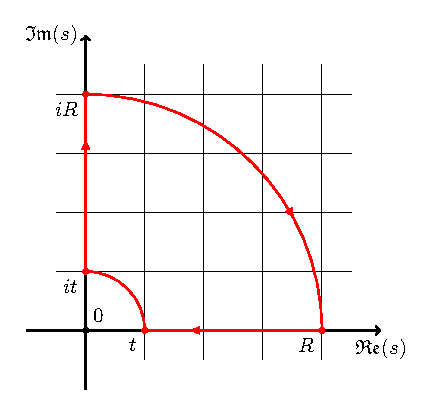
\includegraphics{chapter_Asymptotics/img/contour_quarter}
	\caption{Шлях інтегрування функції $\exp\left(-2 \int\limits_{0}^{u} \frac{e^\tau -1}{\tau(e^\tau - p)} d\tau\right)$}
	\label{fig:contour_phi}
\end{figure}

Нескладно помітити, що для доведення існування інтегралу $\int\limits_{it}^{i\infty}$ достатньо показати, що $\lim\limits_{R \rightarrow \infty}|\int\limits_{K_{R}}| = 0$, адже інтеграл $\int\limits_{t}^{\infty}$ існує через існування $M_{p}(t)$.
А це вже досить нескладно доводиться. \todo{add proof}

Отже, при $t>0$
\begin{equation}
\label{eq:model_laplace_im_ax}
\begin{split}
M_{p}(it) = -\frac{i t^{-2}}{e^{it}-p} \exp \left(2 \int\limits_{0}^{t} \frac{e^{iu} -1}{u(e^{iu} - p)} du\right) \cdot \\
\cdot \int\limits_t^\infty \exp\left(-2 \int\limits_{0}^{u} \frac{e^{i\tau} -1}{\tau(e^{i\tau} - p)} d\tau\right) du.
\end{split}
\end{equation}
Враховуючи, що інтеграл $\int\limits_{1}^{\infty} \frac{1-p}{u(e^{iu} - p)} du$ існує, з \eqref{eq:model_laplace_im_ax} негайно випливає
\begin{equation}
\label{eq:model_laplace_im_ax_asympt}
M_{p}(it) = O(\frac{1}{|t|})
\end{equation}
для $t > 0$. За властивістю перетворення Лапласа $M_{p}(-it) = \overline{M_{p}(it)}$, тому \eqref{eq:model_laplace_im_ax_asympt} виконується і для $t < 0$.
\end{proof}
\end{lem}

Отримали, що
\begin{equation}
\label{eq:uniform_right_as_enhanced}
\lim\limits_{X \rightarrow \infty} \left( m(X) - C_{p} X - \frac{1 - C_{p}}{1 - p} \right) = O\left(\frac{1}{X^{n}}\right) \qquad \forall n \in \mathbb{N}
\end{equation}

Властивість Лапласа..
\begin{equation}
\phi(\overline{u}) = \int_0^\infty M(x) e^{-\overline{u}x} dx = \int_0^\infty M(x) \overline{e^{-sx}} dx = \overline{\phi(u)}
\end{equation}